\documentclass[12pt]{article}


\usepackage{amssymb}
\usepackage{amsmath}
\usepackage{fullpage}
\usepackage{epsfig}
\usepackage{epstopdf}
\everymath{\displaystyle}

\newif\ifans

\anstrue

\begin{document}

\begin{center}
\underline{\LARGE{Chapter 3.6 Practice Problems}}
\end{center}

\noindent EXPECTED SKILLS:

\begin{itemize}

\item Know how to use L'Hopital's Rule to help compute limits involving indeterminate forms of $\frac{0}{0}$ and $\frac{\infty}{\infty}$

\item Be able to compute limits involving indeterminate forms $\infty-\infty$, $0 \cdot \infty$, $0^0$, $\infty^0$, and $1^{\infty}$ by manipulating the limits into a form where L'Hopital's Rule is applicable.

\end{itemize}

\noindent PRACTICE PROBLEMS:

\medskip

\noindent {\bf For problems 1-27, calculate the indicated limit.  If a limit does not exist, write $+\infty$, $-\infty$, or DNE (whichever is most appropriate).  Make sure that L'Hopital's rule applies before using it.  And, whenever you apply L'Hopital's rule, indicate that you are doing so.}

\begin{enumerate}

\item $\lim_{x \rightarrow 3}{\frac{x^2+4x-21}{x^2-7x+12}}$

\ifans{\fbox{$-10$}} \fi

\item $ \lim_{x \rightarrow 0}{\frac{\tan{3x}}{\ln{(1+x)}}}$

\ifans{\fbox{$3$}} \fi

\item $\lim_{x \rightarrow 0}{\frac{\sin{x}-x}{x^2}}$

\ifans{\fbox{$0$}} \fi

\item $\lim\limits_{x\rightarrow 0} \frac{\sin{(6x)}}{\sin{(3x)}}$ 

\ifans{\fbox{$2$}} \fi

\item $\lim_{x \rightarrow 1^-}{\frac{x-1}{x^2-2x+1}}$

\ifans{\fbox{$-\infty$}} \fi

\item $\lim_{x \rightarrow \infty}{\frac{e^{-x}}{x^{-2}}}$

\ifans{\fbox{$0$}} \fi

\item $\lim_{x \rightarrow 0}{\frac{\ln{(\cos{3x})}}{5x^2}}$

\ifans{\fbox{$-\frac{9}{10}$}} \fi

\item $\lim_{x \rightarrow 1}{\frac{\tan^{-1}{x}-\frac{\pi}{4}}{x-1}}$

\ifans{\fbox{$\frac{1}{2}$}} \fi

\item $\lim_{x \rightarrow 0^{+}}{\frac{8^{\sqrt{x}}-1}{1-5^{\sqrt{x}}}}$

\ifans{\fbox{$-\frac{3\ln{2}}{\ln{5}}$}} \fi

\item $\lim_{x\rightarrow 0^{+}}{\frac{5\sin{x}}{\sqrt{x}}}$

\ifans{\fbox{$0$}} \fi

\item $\lim\limits_{x\rightarrow -\infty} \frac{x^3+4x-5}{5x^2-5x-89}$  

\ifans{\fbox{$-\infty$}} \fi

\item $\lim_{x \rightarrow 0}{\frac{\sin^{-1}{(2x)}}{\tan^{-1}{(3x)}}}$

\ifans{\fbox{$\frac{2}{3}$}} \fi

\item $\lim_{x \rightarrow 1}{\frac{\ln{x^2}}{x^2-9}}$

\ifans{\fbox{$0$}} \fi

\item $\lim_{x \rightarrow \infty}{\frac{e^x-e^{-x}}{e^x+e^{-x}}}$

\ifans{\fbox{$1$}} \fi

\item $\lim_{x \rightarrow \frac{\pi}{2}^{+}}{\frac{\ln{\left(x-\frac{\pi}{2}\right)}}{\tan{x}}}$

\ifans{\fbox{$0$}} \fi

\item $\lim\limits_{x\rightarrow 1^-} \frac{x-1}{\arccos{x}}$ 

\ifans{\fbox{0}} \fi

\item $\lim\limits_{x\rightarrow +\infty}\frac{e^{\sqrt{x}}}{x}$ 

\ifans{\fbox{$+\infty$}} \fi

\item $\lim\limits_{x\rightarrow +\infty} xe^{-6x}$ 

\ifans{\fbox{0}} \fi

\item $\lim_{x \rightarrow +\infty}{\frac{\sqrt{4+3x^2}}{2+2x}}$

\ifans{\fbox{$\frac{\sqrt{3}}{2}$}} \fi

\item $\lim\limits_{x\rightarrow 0^+} x \csc{3x}$

\ifans{\fbox{$\frac{1}{3}$}} \fi  

\item $\lim_{x \rightarrow+\infty}\left[\ln{(x+2)}-\ln{(3x+5)}\right]$

\ifans{\fbox{$\ln{\left(\frac{1}{3}\right)}$}} \fi

\item $\lim\limits_{x\rightarrow \infty} 3^{x}7^{-x}$ 

\ifans{\fbox{0}} \fi

\item  $\displaystyle \lim_{x\rightarrow \infty}{\left(\sqrt{x^2-x}-x\right)}$

\ifans{\fbox{$\displaystyle -\frac{1}{2}$}} \fi

\item $\lim\limits_{x\rightarrow 0^+} \tan{x}\sec{x}$ 

\ifans{\fbox{0}} \fi

\item $\lim\limits_{x\rightarrow 0^+} x^{1/x}$ 

\ifans{\fbox{0}} \fi

\item $\lim\limits_{x\rightarrow \infty} \left(1+\frac{2}{x}\right)^{5x}$ 

\ifans{\fbox{$e^{10}$}} \fi

\item $\lim\limits_{x\rightarrow \infty} \left(1-\frac{1}{x}\right)^{-x}$ 

\ifans{\fbox{$e$}} \fi

\newpage

\item Which of the following are indeterminate forms?

\begin{center}
\begin{tabular}{cccc}
$\frac{0}{0}$ & $\frac{0}{\infty}$ & $\frac{\infty}{0}$& $\frac{\infty}{\infty}$
\end{tabular}\\
\medskip
\begin{tabular}{cccc}
$\infty-\infty$ & $\infty+\infty$ & $0 \cdot \infty$ & $\infty \cdot \infty$
\end{tabular}\\
\medskip
\begin{tabular}{cccccc}
$0^0$ & $\infty^0$ & $0^{\infty}$ & $1^\infty$ & $\infty^{\infty}$ & $\infty^{1}$
\end{tabular}
\end{center}

\ifans{\fbox{$\frac{0}{0}$, $\frac{\infty}{\infty}$, $\infty-\infty$, $0 \cdot \infty$, ${0}^{0}$, ${\infty}^{0}$, $1^{\infty}$}} \fi

\item Calculate each of the following limits:

\begin{enumerate}

\item $\lim_{x \rightarrow 0^{+}}{(1+3^x)^{1/x}}$

\ifans{\fbox{$+\infty$}} \fi

\item $\lim_{x \rightarrow 0^{-}}{(1+3^x)^{1/x}}$

\ifans{\fbox{$0$}} \fi

\item $\lim_{x \rightarrow +\infty}{(1+3^x)^{1/x}}$

\ifans{\fbox{$3$}} \fi

\item $\lim_{x \rightarrow -\infty}{(1+3^x)^{1/x}}$

\ifans{\fbox{$1$}} \fi

\end{enumerate}

\item Show that $\lim_{x \rightarrow \infty}{\frac{x^n}{e^x}}=0$ for any positive integer $n$.

\ifans{\fbox{\parbox{1\linewidth}{$\lim_{x \rightarrow \infty}{\frac{x^n}{e^x}}$ is of the indeterminate form $\frac{\infty}{\infty}$, so, we may apply L'Hopital's Rule:
$$\lim_{x \rightarrow \infty}{\frac{x^n}{e^x}}=\lim_{x \rightarrow \infty}{\frac{nx^{n-1}}{e^x}}$$
This new limit is also of the indeterminate form $\frac{\infty}{\infty}$, so, we may again apply L'Hopital's Rule:
$$\lim_{x \rightarrow \infty}{\frac{nx^{n-1}}{e^x}}=\lim_{x \rightarrow \infty}{\frac{n(n-1)x^{n-2}}{e^x}}$$
In fact, we repeat the process until we end up with the following limit:
$$\lim_{x \rightarrow \infty}{\frac{n(n-1)(n-2)\dots(2)(1)}{e^x}}$$
which equals 0.  Thus, $\lim_{x \rightarrow \infty}{\frac{x^n}{e^x}}=0$}}} \fi

\item Find the value(s) of of the constant $k$ which make $f(x)=\left\{\begin{array}{lll}
\frac{\sin{x}-1}{x-\frac{\pi}{2}} & \text{if} & x \neq \frac{\pi}{2}\\
&&\\
k & \text{if} & x=\frac{\pi}{2}
\end{array}\right.$ continuous at $x=\frac{\pi}{2}$.

\ifans{\fbox{$k=0$}} \fi

\item Find all values of $k$ and $m$ such that $\lim_{x \rightarrow 1}{\frac{k+m\ln{x}}{x-1}}=5$

\ifans{\fbox{$k=0$ and $m=5$}} \fi

\item {\bf Multiple Choice:} What is $\displaystyle \lim_{x\rightarrow 1^+} \frac{x}{\ln(x)}$?

\begin{enumerate}

\item $0$\\

\item $1$\\

\item $e$\\

\item $e^{-1}$\\

\item $+\infty$

\end{enumerate}

\ifans{\fbox{E}} \fi

\item {\bf Multiple Choice:} What is $\displaystyle \lim_{x\rightarrow 0}\frac{e^x-1}{\tan(x)}$?

\begin{enumerate}

\item $-1$\\

\item $\ \ 0$\\

\item $\ \ 1$\\

\item $\ \ 2$\\

\item \ \ The limit does not exist.

\end{enumerate}

\ifans{\fbox{C}} \fi

\item {\bf Multiple Choice:} If $\displaystyle \lim_{x\rightarrow +\infty} f(x) =
\lim_{x\rightarrow +\infty} g(x) = +\infty$ and $f'(x)=1$ and $g'(x)=e^x$, what is 
$\displaystyle \lim_{x\rightarrow +\infty}\frac{f(x)}{g(x)}$?

\begin{enumerate}

\item $-1$

\item $\ \ 0$

\item $\ \ 1$

\item $\ \ e$

\item \ \ The limit does not exist.

\end{enumerate}

\ifans{\fbox{B}} \fi

\item A \underline{Regular Polygon} is a polygon that is equiangular (all angles are equal in measure) and equilateral (all sides have the same length).  The diagram below shows several regular polygons inscribed within a circle of radius $r$.

\begin{center}

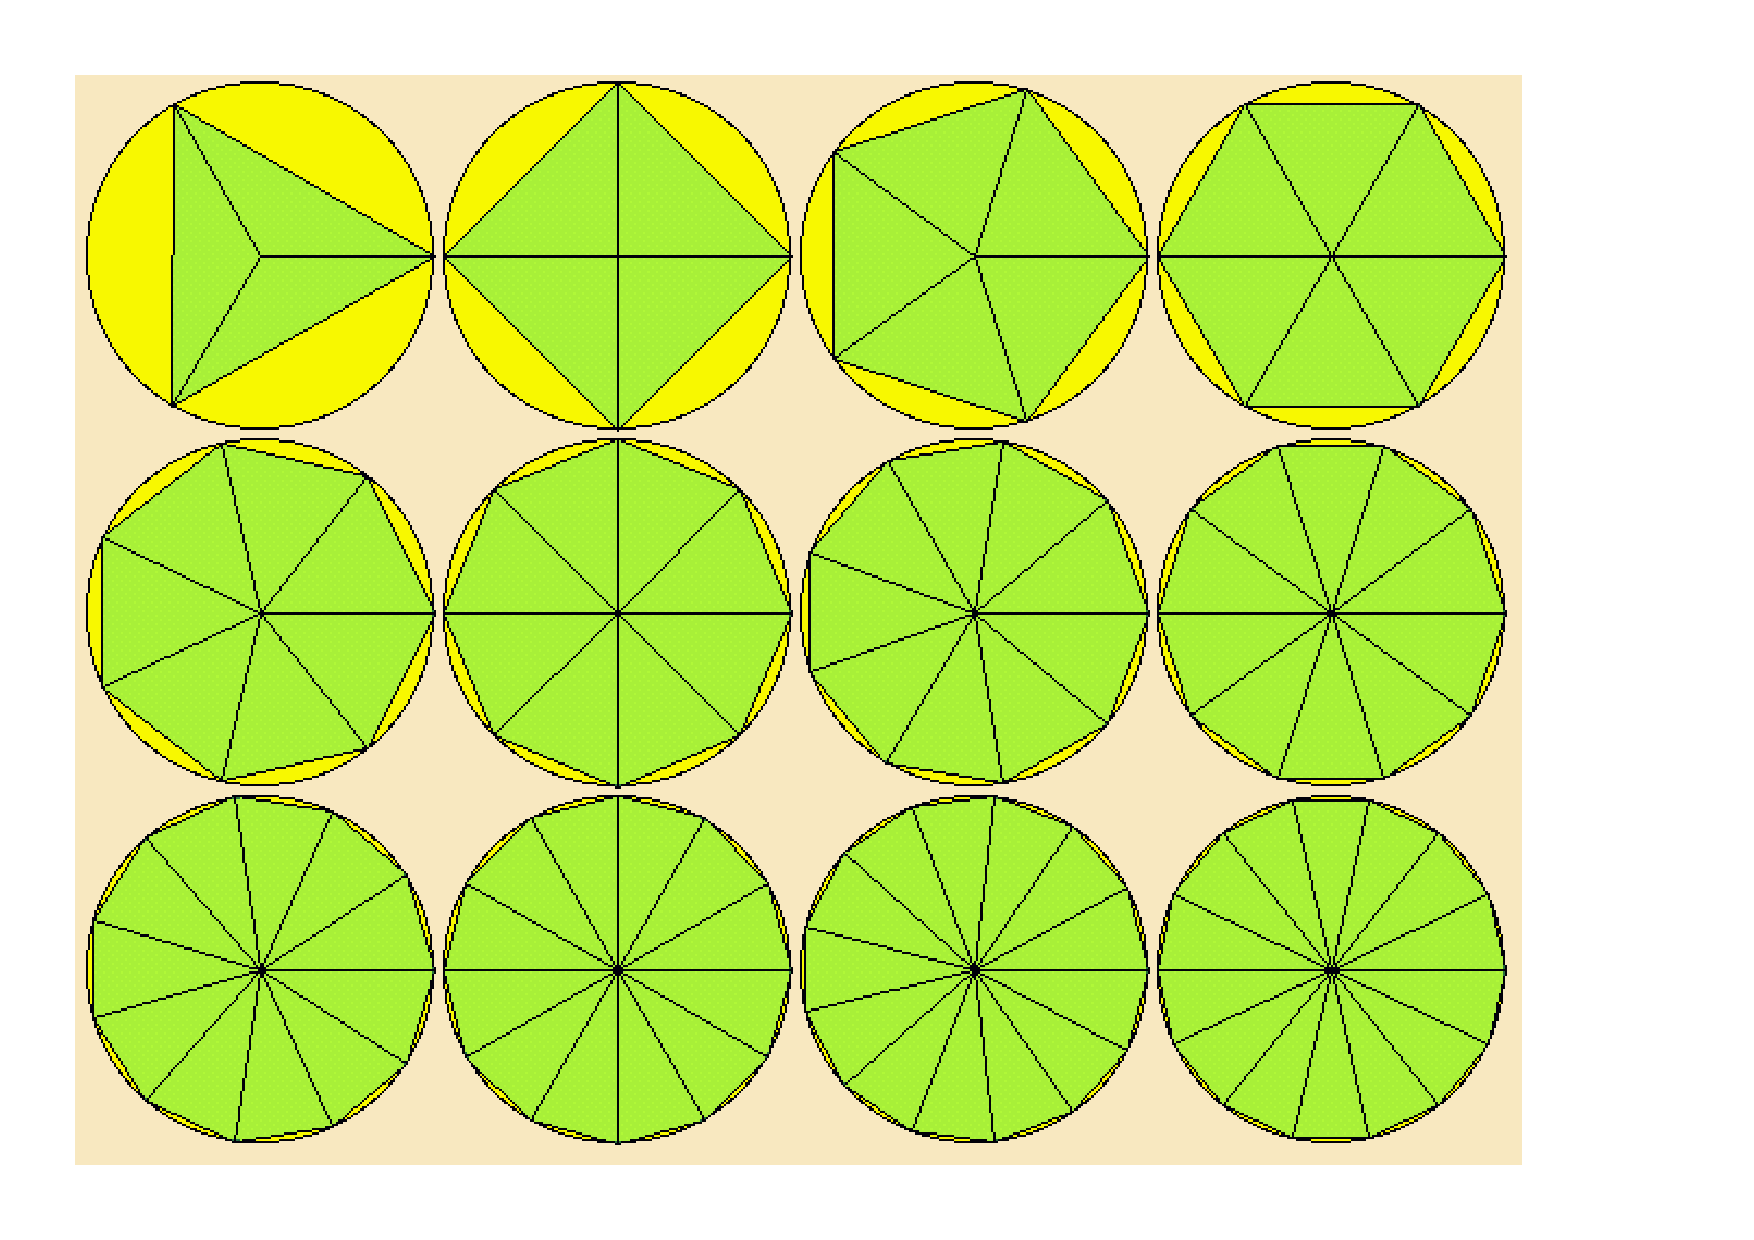
\includegraphics[scale=0.4]{Inscribed.pdf}

\end{center}

\begin{enumerate}

\item Let $A_n$ be the area of a regular $n$-sided polygon inscribed within a circle of radius $r$.  Divide the polygon into $n$ congruent triangles each with a central angle of $\frac{2\pi}{n}$ radians, as shown in the diagram above for several different values of $n$.    Show that $A_n=\frac{1}{2}r^2 \sin{\left(\frac{2\pi}{n}\right)} n$.

\ifans{\fbox{\parbox{1\linewidth}{We begin by examining one of the $n$ triangles, pictured below.
\begin{center}
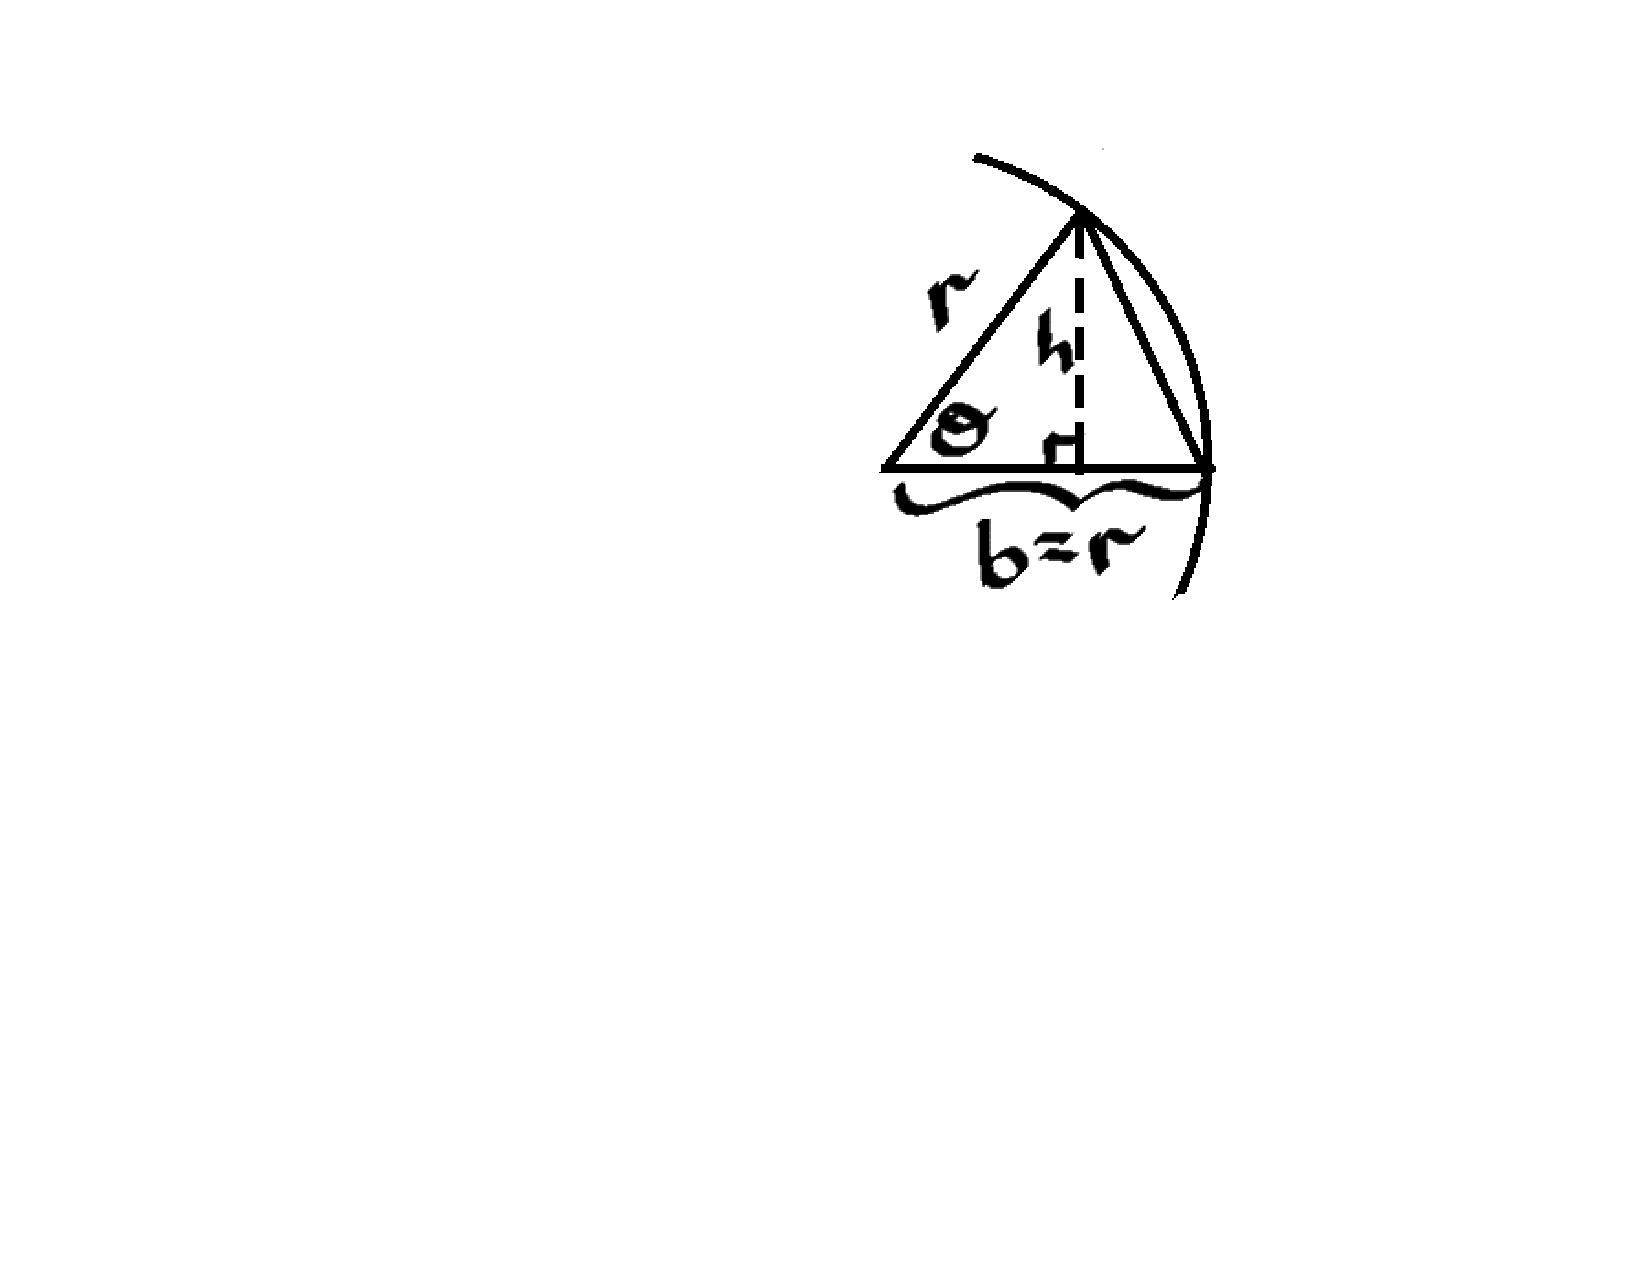
\includegraphics[scale=0.4]{triangle.pdf}
\end{center}
The base of the triangle has a length of $r$.  And, the height of the triangle is $r\sin{\theta}$, where $\theta$ is the central angle, $\frac{2\pi}{n}$.    Thus, the area of one triangle is:
$$A=\frac{1}{2}(r)\left(r\sin{\left(\frac{2\pi}{n}\right)}\right)=\frac{1}{2}r^2\sin{\left(\frac{2\pi}{n}\right)}$$
 But, the polygon is composed of $n$ such triangles.  So, the area of a regular $n$-sided polygon inscribed in the circle of radius $r$ is: 
$$A_n=\frac{1}{2}r^2\sin{\left(\frac{2\pi}{n}\right)}n$$
}}} \fi

\item What can you conclude about the area of the $n$-sided polygon as the number of sides of the polygon, $n$, approaches infinity?  In other words, compute $\lim_{n \rightarrow \infty}{A_n}$.

\ifans{\fbox{$\lim_{n \rightarrow \infty}{A_n}=\pi r^2$}} \fi

\end{enumerate}


\end{enumerate}

\end{document}